\label{chap:Experiments}
This chapter is composed of three parts. The first part talks about FFI experiments, the second part talks about SWIG experiments and the third part talks about Clang experiments. For each part, there is a list of prerequisites and for each experiment, an explanation will be given. This project supports Linux and Mac platform but not for Windows. Source code for the project is in my github\footnote{\url{https://github.com/shenlin192/Projet-de-R-D}}.


\section{FFI Experiments} 

\subsection{Prerequests}
For Node FFI, the following tools are required
    \begin{enumerate}
       \item Install nodejs\footnote{\url{https://nodejs.org/en/}}
       \item Install ffi\footnote{\url{https://github.com/node-ffi/node-ffi}}  
        \item Install DGtal \footnote{\url{https://github.com/DGtal-team/DGtal}}
        \item Install CMake\footnote{\url{https://cmake.org/install/}}
    \end{enumerate}
       
\subsection{How to use?}
    \begin{enumerate}
        \item Clone the repo in github
        \item new a directory in your project path and name it "build" \textit{~your projectPath\$ mkdir build}
        \item go to the "build" directory and run the cmake command \textit{~your projectPath/build\$ cmake ../sourceCode}
        \item \textit{run the make command in newly created "build" directory ~your projectPath/build\$ make}

    After these 4 steps, you have already generated all necessary files for this project.
    Now you can go to the \textit{sourceCode} directory and chose any experiment for testing:

        \item \textit{~your projectPath/sourceCode/experimentName\$ node experimentName.js}
    \end{enumerate}   
       
       
   Our FFI experiments consist of 4 parts. The common goal of these experiments is to use C++ library from within JavaScript by using node-ffi. For each example, I will firstly explain the C++ library that is going to be used, and then explain how to use that library in JavaScript.
       
\subsection{BasicUsage}    

\subsubsection{BasicUsage Library}
  The source code to create a library for this experiment is in path "./sourceCode/cpp/BasicUsage.cpp". It contains:
    \begin{enumerate}
        \item a global function \textit{add} that adds two Integrate and returns the sum 
        \item a class \textit{Rectangle} that contains two private attributes (long and width) and two member functions that calculate its area and perimeter respectively.
        \item a global function \textit{createRectObj} that returns a rectangle object.
        \item a global function \textit{createRectRef} that returns a rectangle pointer.
    \end{enumerate}   
       
\subsubsection{BasicUsage Test}
    The source code to test a library for this experiment is in path "./sourceCode/js/BasicUsage.js". In this test, we have accomplished to
    \begin{enumerate}
        \item Use the function \textit{add} in JavaScript
        \item Create a \textit{Rectangle} object directly in JavaScript
        \item Create a \textit{Rectangle} object in C++ from existing buffer (directly invoke C++ constructor of BasicUsage Library)
        \item Create a \textit{Rectangle} object by using the \textit{createRectObj} function
        \item Create a \textit{Rectangle} object pointer by using the \textit{createRectPtr} function
        \item Encapsulate the creation of C++ object into JavaScript function prototype, so that we can use that object with JavaScript syntax.
    \end{enumerate}
    
    In order to create a C++ class object with Node FFI, we need to firstly define a structure that has the same attributes in JavaScript code as the class in C++ code. The definition of a structure in JavaScript can be done by requiring the "ref-struct" model of Node. Moreover, if we to want to get the reference of any variable defined in JavaScript, we will need the "ref" model of Node.\newline
    In order to use a C++ class's functions, such as its constructors or member functions, in Node-ffi, the reference of an object created by that class should be passed into these functions as their default parameters.

\subsection{Template}       
\subsubsection{Template Library}     
The source code to create a library for this experiment is in path "./sourceCode/cpp/Template.cpp". Its structure is almost the same as the library in BasicUsage experiment expect that it's written in the form of C++ template. We have not rewrite the function add into template form for simplicity of code.

It's a must to implement all the types that we are going to use lately in this library, which means the template classes or functions can not be used directly through node-ffi. Because without specifying types, template functions or template classes cannot be generated into a library's symbol table and thus cannot be found by node-ffi. As for this experiment, type "int" and type "double" are realized.

\subsubsection{Template Test}    
     Source code for testing this experiment is in path "./sourceCode/js/Template". Similar to what we have done for BasicUsage's test, this experiment has:
     
        \begin{enumerate}
            \item Create a \textit{Rectangle} object directly in JavaScript
            \item Create a \textit{Rectangle} object in C++ from existing buffer (directly invoke C++ constructor of Template Library)
            \item Create a \textit{Rectangle} object by using the \textit{createRectObj} function
            \item 
Create a \textit{Rectangle} object pointer by using the \textit{createRectPtr} function
            \item
Encapsulate the creation of C++ object into JavaScript function prototype, so that we can use that object with JavaScript syntax.
        \end{enumerate}
     
     
The main difference is, this time in the JavaScript file, we have to specific which type (int or double) of the template classes or functions is needed. It's worth noting that, in order to distinguish functions or classes that have the same name in C++ source file, the compiler does something called "name mangling", so that after compilation, each function or class will only have a unique name. In our experiment for example, \textit{\_Z13createRectObjii} represents the \textit{Rectangle<int> createRectObj(int a, int b)} function in source code; \textit{\_Z13createRectObjdd} represents the \textit{Rectangle<double> createRectObj(double a, double b)} .
    
     
\subsection{Boost}       
\subsubsection{Boost Library}
Source code to create library for Boost experiment is in path "./sourceCode/cpp/Boost.cpp". Since there are numbers of functions predefined in Boost, we chose only some of them to test if Boost can cooperate with node-ffi. In this experiment, the \textit{timer} and \textit{progress} of Boost are chosen as for testing.

It's worth noting that we do not expose Boost directly to node-ffi. Instead, we created a wrapper function \textit{testBoost} containing the necessary C++ code of Boost for lately using.
\subsubsection{Boost Test}  
     
The source code for boost timer test is in path "./sourceCode/js/Boost.js". The usage of Boost with FFI is the same as the BasicUsage (like calling a normal global function, calling a global variable...). All we need to do is to "include" the Boost library in the C++ file, and then generate a shared library. After that functions defined in Boost can be used easily from JavaScript.     
     


\subsection{2DPoint}
\subsubsection{2DPoint Library}
Source code to create library for Boost experiment is in path "./sourceCode/cpp/2DPoint.cpp".
In the source code, there are two functions, both of which are wrappers that used as the media to invoke DGtal functions.
       
    \begin{lstlisting}[language=c, caption= create2DPoint]
    Point* create2DPoint(int a, int b){
        return new Point(a,b);
    }
    \end{lstlisting}
 Where \textit{Point()} is a built-in constructor of DGtal.   
    
    \begin{lstlisting}[language=c, caption= draw2DPoint]
    void draw2DPoint(Point p1, Point p2){
    Board2D board;
    board << p1<<p2;
    board.saveSVG("draw2DPoint.svg");
}
    \end{lstlisting}


Where \textit{Board2D} is a built-in class of DGtal.    

\subsubsection{2DPoint Test}
Code for this test is in path "./sourceCode/cpp/2DPoint.js". In this test, I've created a point at (3,4) and the other at (1,2) by using the \textit{create2DPoint} function. After that, I draw these two points with the help of \textit{draw2DPoint}. Figure \ref{fig:2DPointResult} shows the result of this test.

     \begin{figure}
        \centering
        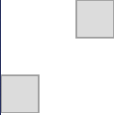
\includegraphics[scale = 0.8]
        {Images/experiments/2DPointsResult.png}
        \caption[2DPoints test result]%
        {2DPoints test result}
        \label{fig:2DPointResult}
    \end{figure}
     
\subsubsection{Go further}     
 Instead of using a wrapper to invoke DGtal functions, it would be much easier and more straightforward to invoke DGtal functions directly.

Use command \textit{\$ objdump -S lib2DPointsLib.so |less}, we found out that the symbol of the constructor after name mangling for a 2 dimension point is:

\begin{lstlisting}
_ZN5DGtal11PointVectorILj2EiNSt3_
_15arrayIiLm2EEEEC1ERKiS6_
\end{lstlisting}

So, we try to use this symbol in the 2DPoint test. It's worth noting
that after name unmangling, we get:
    \begin{lstlisting}
DGtal::PointVector<2u, int, std::__1::array<int, 2ul> >::PointVector(int const&, int const&)
    \end{lstlisting}

Which means it will take two int references as parameters instead of two int variables.

In order to set the value to an int reference, \textit{ref.alloc()} is needed:
    \begin{lstlisting}
    let i1 = ref.alloc(ref.types.int, 2);
    let i2 = ref.alloc(ref.types.int, 9);
    \end{lstlisting}

The output of using the DGtal 2D point constructor is exactly the same as using the \textit{create2DPoint} wrapper function.

     
          
\section{SWIG Experiments}

\subsection{Prerequisites}
    \begin{enumerate}
        \item Install nodejs\footnote{\url{https://nodejs.org/en/}}
        \item Install DGtal \footnote{\url{https://github.com/DGtal-team/DGtal}}
        \item Install SWIG version 3.0 + \footnote{\url{http://www.swig.org/}}
    \end{enumerate}


\subsection{How to use}
The general process of using SWIG's JavaScript interface generators for Node.js are the following 5 steps:

    \begin{enumerate}
        \item Organize all c/c++ logic ( libraries that you want to use) in the form of header files.
        \item Write a SWIG interface file that indicates which libraries should be used
        \item Create a binding file binding.gyp
        \item Run the following commands:\newline
        \textit{\$ swig -c++ -javascript -node mylib.i} for create a wrapper file\newline
        \textit{\$ node-gyp build} for build a node module
        \item After step 4, a node module containing all functions, variables, classes, etc of your c/c++ libraries will be built. And you can start use the generated node module in 
        your JavaScript test file.
    \end{enumerate}


\subsection{Experiments}
The source code of this experiment is in path "./swig".

\subsubsection{Library files}
\textit{global.h}, \textit{rectangle.h}, \textit{templateExample.h} and \textit{TestBoost.h} are the library files for this experiment. \textit{global.h} contains some simple global functions and global variables. The three rest library files are similar to the \textit{BasicUsage Library}, \textit{Template Library} and \textit{Boost Library} in FFI experiments, which are already explained.

\subsubsection{SWIG interface file}
This file indicates which libraries are needed and some more information telling SWIG how to use these libraries. For example, the types of a template should be specified; global functions, as well as global variables, should be declared with the key word \textit{extern}. 


 \begin{lstlisting}[language=c, caption= SWIG interface file]
%module "mylib"

%{
#include "global.h"
#include "rectangle.h"
#include "TestBoost.h"
#include "templateExample.h"
%}

%include "global.h";
%include "rectangle.h";
%include "TestBoost.h";
%include "templateExample.h"
%template (intRectangle) RectangleT<int>;
%template (floatRectangle) RectangleT<float>;

 extern double My_variable;
 extern int fact(int n);
 extern int my_mod(int x, int y);
 extern char *get_time();
}
    \end{lstlisting}

Now, you can run the command \textit{\$ swig -c++ -javascript -node mylib.i}. After that, a wrapper file called \textit{mylib\_wrap.cx} will be created.


\subsubsection{Binding file}
A binding file is used to tell Node.js how to create a node module from a SWIG wrapper (in this example \textit{mylib\_wrap.cxx}) file.

 \begin{lstlisting}[language=c, caption= SWAG interface file]
{
  "targets": [
    {
      "target_name": "mylib",
      "sources": [ "mylib_wrap.cxx" ]
    }
  ]
}

    \end{lstlisting}

Run \textit{\$ node-gyp configure} and then \textit{\$ node-gyp build}. A node module called \textit{mylib} will be built in path "./swig/build/Release/mylib".


\subsubsection{Test file}
The test file is in path "./swig/test.js". I've tried all the libraries mentioned before in this file. All of them work as expected. The following code snippets will show you how to use such a node module.
    \begin{enumerate}
        \item Require the node module that you generated.
        \begin{lstlisting}
    var mylib = require("./build/Release/mylib");
        \end{lstlisting}
        
        \item Usage of global variables and functions
        \begin{lstlisting}
    console.log(mylib.My_variable);
    console.log(mylib.fact(5));
        \end{lstlisting}
        
        \item Usage of a class
        \begin{lstlisting}
     var rectangle = new mylib.Rectangle(5,6);
        \end{lstlisting}
        
        \item Usage of template
        \begin{lstlisting}
    var intRectangle = new mylib.intRectangle(3,4);
    console.log(intRectangle.area());
        \end{lstlisting}
        
        \item Usage of Boost
        \begin{lstlisting}
    var boost = new mylib.TestBoost();
    boost.boostTimer();
        \end{lstlisting}        
    \end{enumerate}

\subsubsection{Go further}
In FFI experiments, I can link the DGtal library ino a shared object by configuring the CMakeLists.txt file. But in SWIG experiments, I still haven't found an equivalent way to link the DGtal library, and thus the 2DPoint experiment is not yet done. I believe SWIG must have provided some options to do this linking but I don't have enough time to do the research.


\section{Clang and LLVM Experiments}
\subsection{Prerequisite}
    \begin{enumerate}
        \item CMake 2.8.6 or later
        \item 30G disk space
        \item 6G swap space
    \end{enumerate}

\subsection{Install}

    \begin{enumerate}
        \item Download llvm:\newline
        \textit{\$ cd where-you-want-llvm-to-live}\newline \textit{\$ svn co http://llvm.org/svn/llvm-project/llvm/trunk llvm}\newline
        
        \item Download Clang:\newline
        \textit{\$ cd where-you-want-llvm-to-live}\newline \textit{\$ cd llvm/tools}\newline
        \textit{\$ svn co http://llvm.org/svn/llvm-project/cfe/trunk clang}\newline
        
        \item Download Compile-RT:\newline
        \textit{\$ cd where-you-want-llvm-to-live}\newline \textit{\$ cd llvm/projects}\newline
        \textit{\$ svn co http://llvm.org/svn/llvm-project/compiler-rt/trunk compiler-rt}\newline
        
        \item Install:\newline
        \textit{\$ cd where you want to build llvm}\newline \textit{\$ svn co http://llvmmkdir build}\newline
        \textit{\$ cd build}\newline
        \textit{\$ cmake -G Unix Makefiles <path to llvm sources>}\newline
        
        \item Make. This will take a very long time:\newline
        \textit{\$ cd where you want to build llvm}\newline \textit{\$ make}\newline

    \end{enumerate}


\subsection{How to increase your swap space?}

As mentioned in the prerequisite, at least 6GB swap space is needed to install LLVM. However, by default, the swap space is the size of memory, which may be less than 6GB. Thus, we need to add swap space manually. The following code shows how to add 4GB to swap space.

    \begin{enumerate}
        \item \textit{\$ dd if=/dev/zero of=/swapfile bs=1024 count=4000000}
        \item \textit{\$ mkswap /swapfile}
        \item \textit{\$ swapon /swapfile}
    \end{enumerate}
    


If you run out of swap space, you will get an error like figure \ref{fig:NotEnoughSwapSpace}: 


    \begin{figure}[H]
        \centering
        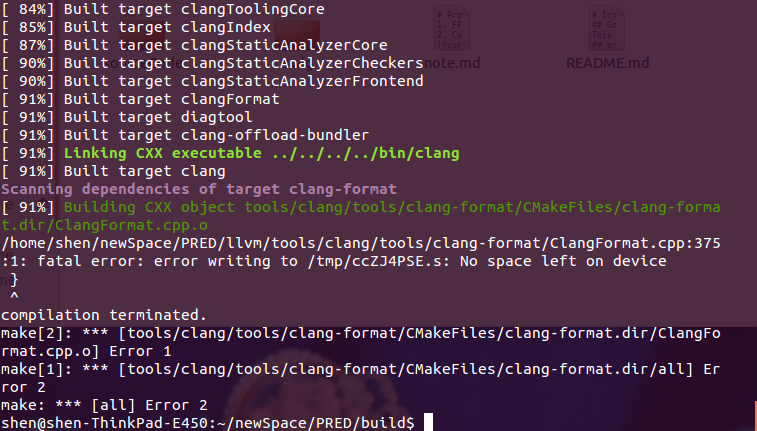
\includegraphics[scale = 0.32]
        {Images/experiments/errorMessage.png}
        \caption[Not enough swap space]%
        {Not enough swap space}
        \label{fig:NotEnoughSwapSpace}
    \end{figure}

\subsection{Display the AST}

The following command can be used to display the AST of a chosen c/c++ file: \newline

\$ clang -Xclang -ast-dump -fsyntax-only <file\_name>

\subsubsection{A simple example}

        \begin{lstlisting}
  int f(int x) {
  int result = (x / 42);
  return result;
}
        \end{lstlisting}     
  
The AST of this example is shown in figure \ref{fig:ClangAST1}        
        
    \begin{figure*}
        \centering
        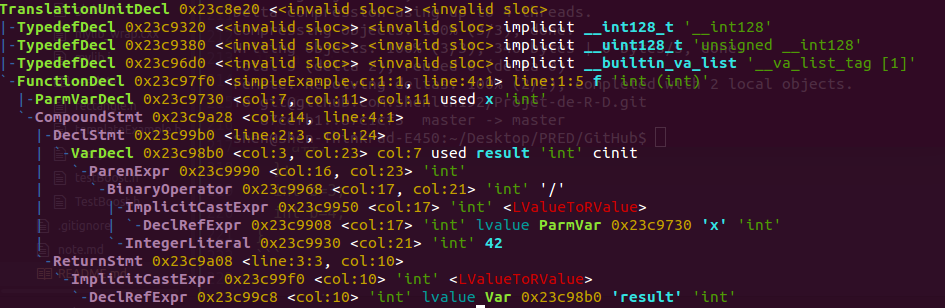
\includegraphics[scale = 0.5]
        {Images/experiments/clangAST1.png}
        \caption[Simple clang AST]%      
{Simple clang AST}
        \label{fig:ClangAST1}
    \end{figure*}
    
    The top-level declaration in a translation unit is always the \textit{translation unit declaration}. In this example, our first user-written declaration is the function declaration of "f". The body of "f" is a \textit{compound statement}, whose child nodes are a \textit{declaration statement} that declares our result variable, and the return statement.
    
\subsubsection{A deliberated error}
\begin{lstlisting}
int a =1;

int function (){
  while (a==1){
    a++;
  };
  int b=3;
  int b=4;
}
 \end{lstlisting}     
  
 The AST result is in figure \ref{fig:ClangAST2}.
 
  \begin{figure*}
        \centering
        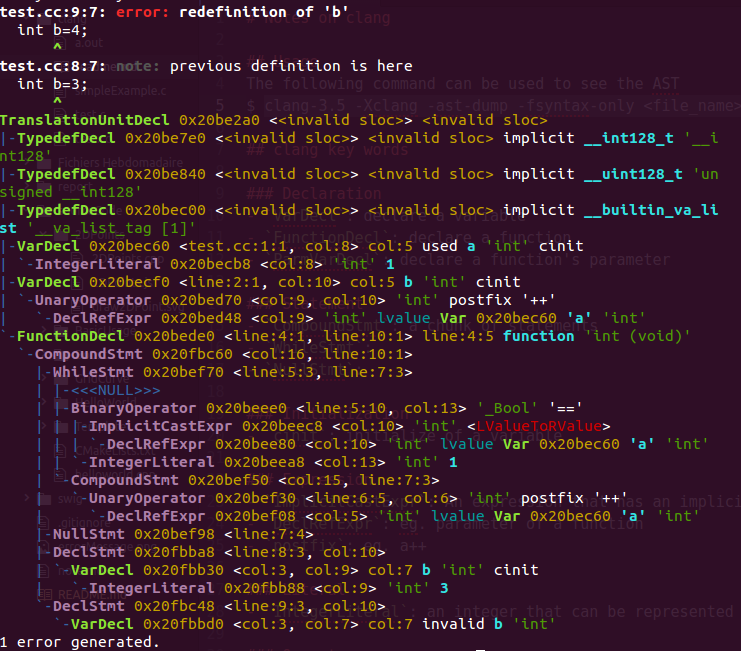
\includegraphics[scale = 0.6]
        {Images/experiments/clangAST2.png}
        \caption[A deliberated error]%
        {A deliberated error}
         \label{fig:ClangAST2}
    \end{figure*}
 
 
 In this example, our deliberately redefined variable b in a function body is detected as an error. The \textit{while} block corresponds to the \textit{WhileStmt}.

I've made notes\footnote{\url{https://github.com/shenlin192/Projet-de-R-D/blob/master/clang/readme.md}} on some basic symbols of Clang. For more information, you need to visit clang's official site\footnote{\url{http://clang.llvm.org/docs/IntroductionToTheClangAST.html}}